% ********** Chapter 1 **********
\chapter{Grundlagen}
\label{sec:background}

Dieses Kapitel stellt bereits vorhandene Technologien vor, welche f"ur die L"osung der Aufgabenstellung relevant sind.
Weiterhin werden Technologien angesprochen, die alternative L"osungen darstellen k"onnten. In diesen F"allen wird kurz
darauf eingegangen, warum sie keine Verwendung finden. Au\ss erdem werden Begrifflichkeiten f"ur den weiteren Verlauf
des Dokumentes eingef"uhrt und erkl"art.

\section{Serviceorientierte Architektur - SOA}
\label{sec:background:soa}
Der Begriff \emph{Serviceorientierte Architektur} oder englisch \emph{Service Oriented Architecture}, auch \emph{diensteorientierte Architektur},
beschreibt ein Softwarearchitekturkonzept welches versucht durch lose Kopplung autarker Module - sogenannter Services -
Gesch"aftsprozesse besser und schneller abbilden zu k"onnen als traditionelle Architekturen. Diese Services bilden
einzelne Schritte der Gesch"aftsprozesse nach und bieten standardisierte Schnittstellen an, "uber welche sie angesprochen
werden k"onnen. Dienste werden von einem \emph{service provider} angeboten und von einem \emph{service consumer}
mittels eines \emph{service request} angesprochen; der Dienst antwortet mittels eines \emph{service response}.
Die Koppelung mehrerer Dienste wird "uber ein oder mehrere Protokolle wie zum Beispiel \emph{SOAP}
\footnote{Simple Object Access Protocol, XML-basiertes Protokoll zum Nachrichtenaustausch "uber Rechnernetzwerke, siehe \ref{sec:background:soap}}
oder \emph{RMI}
\footnote{Remote Method Invocation, API zum Aufruf entfernter Methoden, siehe \ref{sec:background:rmi}}, 
aber auch durch den Einsatz ganzer dienstorientierter Technologien
wie \emph{CORBA} \footnote{
Common Object Request Broker Architecture - objektorientierte, plattformunabh"angige Middleware die Protokolle und Dienste
spezifiziert, die das erstellen verteilter Anwendungen in heterogenen Umgebungen vereinfachen soll. CORBA wird von
der Object Management Group entwickelt, siehe \cite{OMGHP}}
oder \emph{Enterprise Java Beans} (vgl. \ref{sec:background:rmi} und \ref{sec:chap2}) erreicht. 
Aufgrund der Plattformunabh"angigkeit solcher Technologien eignet sich eine solche Architektur auch besonders um vorhandene
Strukturen miteinander zu verbinden, und die Heterogenit"at verschiedener Systeme zu "uberwinden.
Ein weiterer wesentlicher Aspekt von SOA ist die Kapselung des Zugriffes
auf persistente Daten durch einzelne Services, welche als einzige schreibend auf diese Daten zugreifen k"onnen, was 
die Gew"ahrleistung der Konsitenz solcher persistenter Daten erheblich vereinfacht. 
Der Begriff SOA fasst eine Vielzahl von Technologien und Herangehensweisen zusammen, und ihn an dieser Stelle komplett zu 
erl"autern w"urde den Rahmen des Dokumentes sprengen, interessierte Leser sollten eines der zahlreichen B"ucher
zu diesem Thema konsultieren, beispielsweise \cite{SOABOOK} und \cite{SOABOOK2}.

\section{Skriptsprachen}
\label{sec:background:script}

Als Skriptsprachen bezeichnet man Programmiersprachen, welche urspr"unglich vor allem zur L"osung
kleinerer Programmieraufgaben entwickelt wurden. Sie stellen im Allgemeinen keine so hohen formalen 
Anspr"uche an den Programmierer wie "'vollst"andige"' Programmiersprachen, so verzichten sie
beispielsweise oft auf den Deklarationszwang von Variablen. Weitere, h"aufig bei
Skriptsprachen anzutreffende Merkmale sind unter anderem die dynamische, beziehungsweise oft auch komplett 
fehlende Typisierung von Variablen, die automatische Speicherverwaltung, und vor allem das
"ubersetzungsfreie Ausf"uhren - die Programme werden \emph{interpretiert}. Dies f"uhrt allerdings
dazu, dass Skriptsprachen oft nicht so effizient sind wie direkt "ubersetzte Programme. Weiterhin
treten so viele Fehler die ein Compiler finden, beziehungsweise komplett verhindern w"urde erst zur
Laufzeit und somit m"oglicherweise im Produktivbetrieb auf.
Der "Ubergang zwischen klassischen Programmiersprachen und Skriptsprachen ist heute jedoch flie\ss end: 
Sprachen wie beispielsweise Java bieten ebenfalls eine automatisierte Speicherverwaltung und werden nicht
direkt in Maschinencode sondern in Bytecode "ubersetzt, welcher dann interpretiert wird, w"ahrend 
Skriptsprachen wie Python oder Ruby teilweise sehr hohe formale Anspr"uche stellen und sehr robust sind.
Die klassischen Einsatzgebiete von Skriptsprachen werden heute erweitert durch Webanwendungen und
\emph{rapid prototyping}\footnote{
Das Entwickeln eines Prototyps des zu erstellenden Softwaresystems, ohne die vollen Anspr"uche an Umfang und
Qualit"at erf"ullen zu wollen.
}.
Sie werden auch gerne als sogenannte \emph{glue languages}
- als verbindender "'Kleber"' zwischen verschiedenen Systemen, Programmen und Programmiersprachen -
eingesetzt. Skriptsprachen sind au\ss erdem beliebt um Softwaresysteme f"ur weniger versierte Anwender
leicht erweiterbar zu machen, indem sie eine kontrollierte, leicht erlernbare und trotzdem 
ausreichend m"achtige Umgebung bieten, in der dieser Anwender der Applikation eigene Funktionalit"at 
hinzuf"ugen kann.
Im weiteren Verlauf dieses Dokumentes werden Programme, welche in einer Skriptsprache geschrieben sind 
auch kurz als \emph{Skripte} bezeichnet. Beispiele weitverbreiteter Skriptsprachen sind das in dieser
Arbeit behandelte \emph{PHP}, der Klassiker \emph{Perl} sowie die neueren Sprachen \emph{Ruby} und \emph{Python}.

\subsection{PHP}
\label{sec:background:php}

Das PHP-Manual \cite{PHPMAN} schreibt "uber PHP: "`PHP (Akronym f"ur "'PHP: Hypertext Preprocessor"') 
ist eine weit verbreitete und f"ur den allgemeinen Gebrauch bestimmte Open Source Skriptsprache, 
welche speziell f"ur die Webprogrammierung geeignet ist, und in HTML eingebettet werden kann."'

Das heutige PHP entstand aus den urspr"unglich 1994 von \emph{Rasmus Lerdorf} in C geschriebenen und "uber CGI
\footnote{Common Gateway Interface, Schnittstelle zwischen einem Webserver und einem externen Programm, siehe \ref{sec:background:cgi}}
ausgef"uhrten "'Personal Home Page Tools"'. 1995 wurden diese von Lerdorf erstmals als "'PHP/FI"' ver"offentlicht,
nachdem er sie mit einem Interpreter f"ur Formulardaten ausgestattet hatte.
1997 schrieben die beiden israelischen Entwickler \emph{Zeev Suraski} und \emph{Andi Gutmans} den Parser neu und
schufen so die Grundlage f"ur PHP 3, welches 1998 ver"offentlicht wurde. Diese Version bot auch 
erstmals grundlegende M"oglichkeiten zur objektorientierten Programmierung, allerdings war die gesamte 
Standardbibliothek noch prozedural angelegt.
Suraski und Gutmans fingen daraufhin an den Kern von PHP neu zu schreiben, welcher seit 1999 als \emph{Zend Engine}
von der neu gegr"undeten \emph{Zend Technologies} vertrieben wird. Im Mai 2000 wurde PHP 4 der
"Offentlichkeit als erstes PHP vorgestellt, welches die Zend Engine in der Version 1.0 nutzte (siehe auch \cite{ZENDENGINE}).
PHP 4 wird bis heute von Zend unterst"utzt und wird bei 1\&1 noch produktiv eingesetzt, obwohl es noch sehr unter den
mangelhaften F"ahigkeiten zur Objektorientierung von PHP 3 leidet. Es werden weder Kapselung der Daten,  
zum Beispiel durch private Variablen, noch Destruktoren oder Fehlerbehandlung "uber Exceptions unterst"utzt.
Im Juli 2004 wurde PHP 5 zusammen mit der Zend Engine II ver"offentlicht und bot lang erwartete Features wie
robuste Objektorientierung, native SOAP-Unterst"utzung (siehe \ref{sec:background:soap}), 
Iteratorkonstrukte und Exceptions. Zu diesem Zeitpunkt wird an der n"achsten PHP Version 6 entwickelt. Diese Version
befindet sich allerdings noch in einem sehr fr"uhen Stadium, und es wird sowohl Zend-intern als auch "offentlich noch heftig 
"uber die Richtung debatiert, in die PHP sich in Zukunft bewegen soll.  

PHP Quelltext wird - wie bei vielen Skriptsprachen, zum Beispiel Perl - nicht kompiliert sondern zur Laufzeit ausgewertet und interpretiert.
Die Sprache bietet nur einige wenige Datentypen, welche alle in einer einzigen Art von Variable gespeichert werden
(\emph{weak typing}) - sprich Variablen k"onnen zur Laufzeit ihren Typ "andern, 
was von vielen als ein weiterer Kritikpunkt angesehen wird, da es zu Laufzeitfehlern kommen kann die in anderen 
Sprachen schon von vorneherein durch den Compiler ausgeschlossen sind
\footnote{
siehe hierzu auch den Artikel von Bruce Eckel, zu finden unter \cite{TYPING}
}.
Dieser Variablentyp wird \emph{zval} genannt, und ist auf C-Ebene ein \texttt{struct}, der neben einem Feld das den aktuell 
gespeicherten Typ vorh"alt einen \texttt{union} enth"alt, in dem der eigentliche Wert der Variable gespeichert wird.
Ein weiteres Problem ist, dass der Sprachumfang von PHP durch Dritte mittels \emph{Extensions}
genannter Erweiterungen erweitert werden kann, und wird. Dies muss allerdings zur Kompilierzeit von PHP geschehen, was wiederum
dazu f"uhrt, dass verschiedene PHP-Installationen verschiedenen Funktionsumfangs sein k"onnen. 
Dadruch dass die Extensions meist durch Dritte entwickelt werden kann es vorkommen, dass
verschiedene gleichartige Extensions - zum Beispiel die Datenbankerweiterungen zu MySQL\footnote{
Weitverbreitete Open Source Datenbank, siehe \cite{MySQL}} und Sybase\footnote{
Bei 1\&1 neben MySQL haupts"achlich eingesetzte Datenbank, siehe \cite{SYBASE}} - nicht
nur unterschiedliche Methodensignaturen, sondern auch unterschiedliches Verhalten "ahnlicher Methoden haben.

Der Einsatz von PHP innerhalb von 1\&1 ist historisch vor allem dadurch zu erkl"aren, dass zun"achst keine 
konkurrenzf"ahigen Technologien existierten, und sp"ater erstens schon sehr viel in diese Technologie investiert
worden war und zweitens etwaige technischen Nachteile von PHP durch im Unternehmen vorhandenes Know-How sehr gut
ausgeglichen werden konnten.

Die Tatsache, dass PHP urspr"unglich als reine Web-Programmiersprache konzipiert wurde ist heute noch deutlich sichtbar, 
unter anderem an 
Variablen und Funktionen, die ohne eine Web-Umgebung keinen Sinn ergeben. Vor allem macht sie sich aber in der Zend-Engine selbst,
bemerkbar, da
an vielen Stellen noch zwischen Modul (dem Interpreter) und Request (dem einzelnen Zugriff auf eine URL) unterschieden
wird. Dies mag auch der Grund daf"ur sein, dass keine dem Application Server vergleichbare Technologie f"ur PHP existiert.
F"ur PHP ist das Ausf"uhren einer alleinstehenden Applikation eher die Ausnahme als die Regel.

Dennoch erfreut sich PHP heute sehr gro\ss er Beliebtheit, wohl vor allem aufgrund der hohen Anzahl von Webservern,
die ihren Benutzern die M"oglichkeit bieten mittels PHP dynamische Inhalte zu generieren. Obwohl Perl -
als gr"o\ss ter "'Konkurrent"' zu PHP - 
wohl eine "ahnlich hohe Verbreitung hat schreckt gerade viele Einsteiger die komplizierte Syntax dieser Sprache ab.


\subsection{Common Gateway Interface - CGI}
\label{sec:background:cgi}

Skriptsprachen im Allgemeinen und PHP im Besonderen sind sehr stark mit dem \emph{Common Gateway Interface} verbunden.
CGI erlaubt einem Webserver (zum Beispiel dem \emph{apache.org HTTP Server} \cite{APACHEHP}) externe Programme zu nutzen, um
neben statischen Inhalten auch die Generierung dynamischer Inhalte zu erm"oglichen. 
Hierzu wird der Zugriff (engl. \emph{Request}) mittels
Umgebungsvariablen formalisiert und an ein externes Programm weitergegeben, welches f"ur jeden Zugriff neu gestartet wird.
Diese Programme sind oftmals in Skriptsprachen geschrieben, 
auch weil diese oftmals sehr komfortable Methoden besitzen um Strings zu manipulieren.
CGI wurde mit \emph{FastCGI} weiterentwickelt, FastCGI-Programme werden nicht f"ur jeden Request neu gestartet, sondern werden
im Speicher gehalten und nur mit den neu ankommenden Requests versorgt. Einem "ahnlichen Prinzip folgen Server-Module, nur sind
diese keine ausf"uhrbaren Programme, sondern Programmbibliotheken und werden direkt in den Webserver geladen.

\section{XP-Framework}
\label{sec:background:xp}

Das XP-Framework \cite{XPHP} (XP) ist der Hauptgrund weshalb - trotz der sehr mangelhaften M"oglichkeiten zur 
Objektorientierung - bei 1\&1 PHP 4 noch an vielen Stellen eingesetzt wird. XP ist ein modulares Framework, welches
dem Anwender die Entwicklung jeglicher Anwendung in PHP erleichtern soll; es wird seit 2001 nach streng 
objektorientierten Kriterien und mittels eines agilen Prozesses haupts"achlich bei 1\&1 hausintern entwickelt,
ist aber komplett open source und wird unter der \emph{BSD-Lizenz}
\footnote{Die BSD-Lizenz ist eine sehr liberale Open Source Lizenz, siehe \cite{BSDLICENCE}}
vertrieben.
Eine zentrale Motivation f"ur die Entwicklung des XP-Frameworks war die "Uberwindung der angesprochenen
Defizite von PHP 4. Daher wurde unter anderem ein eigener Exception-Mechanismus, Methoden zum dynamischen
Laden und zur Reflektion von Klassen, OO-Mapping von Datenbankzugriffen, sowie Abl"aufe zur sauberen 
Trennung von Logik und Pr"asentation entwickelt. Desweiteren enth"alt XP "Aquivalente zu sehr vielen Java-Standardklassen.
Durch sorgf"altige, an Javadoc \cite{JAVADOC} angelehnte Dokumentation im Sourcecode wird versucht die mangelnde
Typisierung in PHP zu "uberwinden, was M"oglichkeiten zur automatischen Generierung von API-Dokumentation und zum
Beispiel WSDLs\footnote{
WSDL ist eine Webservicebeschreibungssprache, siehe \cite{WSDLSPEC}}
f"ur SOAP er"offnet.

Alles in allem erlaubt das XP-Framework die Vorteile von PHP wie kurze Entwicklungszeiten und einfache 
Programmierung zu nutzen ohne auf die Vorteile der Objektorientierung zu verzichten.
Viele dieser Funktionen setzen allerdings voraus, dass der ausf"uhrende PHP-Interpreter bestimmte Erweiterungen bereitstellt,
ohne die beispielsweise das Transformieren von XML mittels XSL, die FTP- und Mailfunktionalit"at oder auch
der Zugriff auf Datenbanken wie MySQL oder Sybase nicht m"oglich w"aren.
An einer Portierung des Frameworks nach PHP 5 wird zwar schon l"anger gearbeitet, allerdings gestaltet sich dieses Vorhaben
aufgrund der ge"anderten Verhaltensweisen der Programmiersprache bez"uglich Referenzen sowie der von den Entwicklern der Zend-Engine
etwas unbedacht eingef"uhrten Exceptions schwierig. Desweiteren werden PHP st"andig neue Standardklassen
hinzugef"ugt was ob der fehlenden Namensr"aume zu Kollisionen mit Klassen des Frameworks f"uhrt.
Es existieren fertige, PHP 5 kompatible Versionen aller Basisklassen. Zum Zeitpunkt der Erstellung dieses
Dokumentes werden neue Anwendungen 
in PHP 5 entwickelt, viele "altere Applikationen laufen aber weiterhin in PHP 4 und m"ussen daher auch weiterhin
gewartet werden.


\section{SOAP}
\label{sec:background:soap}
SOAP stand urspr"unglich f"ur \emph{\textbf{S}imple \textbf{O}bject \textbf{A}ccess \textbf{P}rotocol},
heute ist SOAP nur noch ein Eigenname.
SOAP ist ein Protokoll, welches den Austausch XML-basierter Nachrichten "uber ein Rechnernetzwerk - "ublicherweise
mittels HTTP - erlaubt. SOAP-Implementierungen sind heute f"ur fast jede Programmiersprache verf"ugbar. SOAP wird
ab PHP Version 5 inh"arent unterst"utzt; auch innerhalb des XP-Frameworks stehen entsprechende Klassen zur Verf"ugung.
SOAP entstand aus einer Zusammenarbeit von \emph{Dave Winer} und \emph{Microsoft}, im Jahre 2000 schlossen sich 
weitere Firmen, darunter IBM, der Entwicklungsgruppe an und reichten den Entwurf zu SOAP 1.1 beim 
\emph{World Wide Web Consortium} (W3C) zur Weiterentwicklung ein, welches 2003 den aktuellen Standard SOAP 1.2
ver"offentlichte.
Eine SOAP Nachricht besteht lediglich aus einem \emph{SOAP-Envelope} welcher wiederum ein (optionales) \emph{Header}-Element
und ein \emph{Body-Element} enth"aelt und verwendete Namesr"aume festlegt \cite{SOAPSPEC}. Die eigentlichen Nutzdaten sind
im Body-Element untergebracht und m"ussen vom Empf"anger der Nachricht interpretiert werden, w"ahrend im Header-Element Metadaten
zur Nachricht enthalten sind, welche ebenfalls von den empfangenden Stationen interpretiert werden m"ussen. Diese sehr weit gefasste
Spezifikation erlaubt es sehr flexible Anwendungen zu entwickeln, allerdings bringt SOAP auch einige Nachteile mit sich:\\
Aufgrund der Verwendung von XML zur Kodierung der zu "ubertragenden Informationen vervielfacht sich das "Ubertragungsvolumen
deutlich was nicht nur Probleme mit der verwendeten Bandbreite verursacht, sondern auch
erhebliche Mengen an Rechenleistung bei der Generierung und Verarbeitung der Nachrichten erfordert. Ein weiterer Kritikpunkt ist
die mangelhafte und zum Teil sich selbst widersprechende Spezifikation selbst, was unter anderem dazu f"uhrt dass mittels verschiedener
Software (\emph{tool-chains}) erzeugte SOAP-Services und -Anwendungen nicht ohne h"andisches Eingreiffen des Entwicklers miteinander kommunizieren 
k"onnen. Um dieses Manko zu beheben wurde eigens die \emph{Web Services Interoperability Group} \footnote{
Die WS-I wird von vielen Unternehmen unterst"utzt die darauf angewiesen sind, dass Web-Services plattform- und programmiersprachen"ubergreifend
funktionieren, weswegen ihre Vorschl"age mittlerweile von weiten Teilen der Industrie als normgebend angesehen werden,
siehe \cite{WSIHP}
}
gegr"undet, eine Organisation, die versucht den Standard zu standardisieren. Allein Existenz einer solchen Organisation zeugt von der
Mangelhaftigkeit der urspr"unglichen SOAP-Spezifikation.
Da die Spezifikation keine Aussagen "uber Transaktionalit"at trifft m"usste solches Verhalten - falls gew"unscht - von jeder Applikation selbst
definiert und vom Benutzer implementiert werden, was dazu f"uhrt dass es in der Praxis unm"oglich ist Anwendungen mittels SOAP zu
verwirklichen welche Transaktionen ben"otigen w"urden. Auch ist nicht standardisiert wie dynamisch Daten "uber bei einem Server verf"ugbare
Dienste erlangt werden k"onnen. Zu diesem Zweck wird meist ein \emph{WSDL}-Dokument \cite{WSDLSPEC} eingesetzt, allerdings wird auch an diesem
Standard viel Kritik ge"ubt, er beschreibt beispielsweise weder wie ein \emph{WSDL}-Dokument f"ur einen speziellen Dienst zu beziehen ist,
noch enth"alt ein solches Dokument Informationen, die "uber die syntaktische Beschreibung des Dienstes hinausgehen.
Ein weiteres SOAP-spezifisches Problem ist,
dass kein Mechanismus definiert wird, "uber welchen Nachrichten aktiv an einen Teilnehmer "ubermittelt werden k"onnen, weshalb dieser
st"andig "uberpr"ufen muss, ob neue Daten f"ur ihn vorliegen ("'polling"').

\section{XML-RPC}
\label{sec:background:xmlrpc}
XML-RPC (vom englischen \textbf{R}emote \textbf{P}rocedure \textbf{C}all) ist ein Vorg"anger von SOAP, und setzt - wie schon
aus dem Namen hervorgeht - ebenfalls XML zur Kodierung der zu "ubertragenden Informationen ein. Im Gegensatz zu den meisten anderen
Sytemen die den Aufruf entfernter Methoden erlauben ist XML-RPC sehr simpel gehalten und definiert nur einige wenige
Datentypen. Diese sehr schlanke Spezifikation verhindert zwar, dass die zu "ubertragenden Nachrichten wie bei SOAP zu sehr 
aufgebl"aht werden, allerdings schr"ankt sie auch die m"ogliche Komplexit"at der zu versendenden Strukturen stark ein.
XML-RPC eignet sich folglich gut um einfache Dienste anzubieten. F"ur komplexe Anwendungen hingegen w"urde man sich eher 
f"ur eine fortgeschrittenere Technologie entscheiden. Nichtsdestotrotz sollte es an dieser Stelle erw"ahnt werden.

\section{Java Enterprise Edition - Java EE}
\label{sec:background:jboss}
\label{sec:background:rmi}
Java EE erweitert den Java Standard unter anderem um Funktionalit"at, die es dem Entwickler erlaubt verteilte, transaktionsbasierte und
mehrschichtige (\emph{multitier}) Anwendungen zu entwickeln (siehe auch \cite{JEEHP}). Hierzu spezifiziert Java EE mehrere Komponenten, wie unter anderem
\emph{Enterprise Java Beans (EJBs)}, \emph{Servlets} und \emph{Java Server Pages (JSPs)} und APIs sowie klare Schnittstellen zwischen
diesen Komponenten. EJBs im besonderen sind standardisierte Komponenten innerhalb einer Java EE Architektur, mit denen verschiedene
Dienste umgesetzt werden, die f"ur die Gesch"aftslogik einer Anwendung notwendig sind. EJBs existieren in verschiedenen Auspr"agungen, die
verschiedene Klassen von Anwendungsf"allen abdecken:
\begin{description}
\item{\textbf{Session Bean}} - Session Beans bilden Vorg"ange ab, insbesondere solche die der Nutzer an einem System durchf"uhrt. Session Beans
    implementieren immer ein Service-Interface, "uber dessen Methoden der Benutzer mit dem System interagieren kann. 
    Man unterscheidet zustandslose (stateless) und zustandsbehaftete (stateful) Session Beans. Eine Stateful Session Bean kann -
    im Gegensatz zu einer Stateless Session Bean - Daten "uber mehrere Aufrufe hinweg speichern, wobei diese Daten immer
    einem bestimmten Nutzer zugeordnet bleiben.
\item{\textbf{Message Driven Bean}} - Message Driven Beans erm"oglichen eine asynchrone Kommunikation innerhalb eines Java EE Systems, indem
    sie auf JMS\footnote{Java Message Service, API von Sun zum Austausch von Nachrichten zwischen zwei oder mehr Clients, siehe\cite{JMSHP}}
    -Nachrichten, die in bestimmten Warteschlangen vorgehalten werden, reagieren.
\item{\textbf{Entity Bean}} - Entity Beans bilden die persistenten Daten, beispielsweise Felder einer Datenbank, innerhalb eines Systems ab und
    bieten Methoden diese Daten aufzufinden, zu ver"andern und wieder abzuspeichern. In der neuesten EJB-Spezifikation\footnote{
    EJB 3.0 Specifications, siehe \cite{EJBHP}} kommt Entity Beans eine weitaus weniger wichtige Bedeutung zu, da die Datenpersistenz nun
    mittels ganz normaler Java-Objekte (POJOs), deren Persistenzeigenschaften vom sogenannten \emph{EntityManager} realisiert werden, abgebildet wird.
    Die Entity Bean als Datentransferobjekt wird somit nicht mehr ben"otigt.
\end{description}
Diese Technologien ben"otigen einen sogenannten \emph{Java Application Server} welcher die n"otige Infrastruktur
f"ur Sicherheit, Transaktionsmanagement, Kommunikation und vielem mehr unabh"angig von Betriebssystem, Netzwerk- und Rechnerarchitektur
bereitstellt. Der Application Server ist in mehrere Module (sogenannte \emph{Container}) unterteilt, welche als Laufzeitumgebungen f"ur einzelne
Komponenten fungieren - so werden zum Beispiel EJBs im EJB-Container ausgef"uhrt. Zum Aufruf von Methoden entfernter Objekte bietet Java 
RMI (\textbf{R}emote \textbf{M}ethod \textbf{I}nvocation) an, was entweder "uber ein eigenes Protokoll oder aber "uber IIOP gefahren werden kann.
RMI ist ein bin"ares Protokoll, was den erzeugten Overhead im Vergleich mit SOAP erheblich reduziert.
Ausserdem bietet RMI Transaktionssicherheit. RMI eignet sich deswegen besser f"ur 
komplexe Anwendungen, bei denen auch die Antwortzeit eine Rolle spielt. RMI hat sich auch innerhalb der 1\&1 als bevorzugtes Protokoll 
etabliert um Dienste miteinander zu verkn"upfen. Leider existiert keine PHP-Implementierung, und die Komplexit"at und die bin"are Natur des
Protokolls machen eine Eigenentwicklung einer solchen Implementierung fast unm"oglich.


\section{Enterprise Application Server Connectivity - EASC}
\label{sec:background:easc}
EASC ist eine haupts"achlich von Christian Gellweiler im Rahmen einer Diplomarbeit f"ur 1\&1 entwickelte 
"'Protokollbr"ucke welche es PHP-Applikationen erlaubt RMI-Aufrufe mittels eines Stellvertreters auszuf"uhren, welcher
Daten und Anweisungen "uber ein generisches Protokoll erh"alt."' \cite{EASC}\\
Dieser Proxy kommuniziert mit dem innerhalb des J2EE-Application-Servers ausgef"uhrten sogenannten \emph{EASC Service-MBean} mittels
eines speziellen Protokolls, welches die Serialisierung und "Ubertragung von Daten und Objekten erlaubt.
Die Erzeugung der Proxyklassen ("'Stub"') "ubernimmt ein spezielles Programm, welches es dem Entwickler erlaubt aus einer in Java geschriebenen
Remote Interface Klasse des aufzurufenden Enterprise Beans eine "aquivalente PHP-Klasse zu erzeugen.
Wird innerhalb von PHP eine Methode des Stubs aufgerufen, so serialisiert dieser diesen Aufruf und "ubermittelt diesen mittels des EASC-Protokolls
an die MBean. Die MBean deserialisiert diesen, und t"atigt die seinerseits n"otigen RMI Aufrufe.
In der Gegenrichtung werden R"uckgabewerte und Fehlermeldungen - wiederum "uber besagtes Protokoll - zur"uckgeliefert.
EASC erlaubt es also einer komplett in PHP geschriebenen Anwendung auf J2EE-Dienste zuzugreifen, welche andernfalls nur
erreichbar w"aren w"urde diese Anwendung selbst in einer solcher Umgebung ausgef"uhrt. Allerdings bietet EASC keine M"oglichkeit
selbst Dienste in PHP zu entwickeln, die ihrerseits aus einer J2EE-Umgebung mittels RMI aufgerufen werden k"onnen.
\begin{figure}[h]
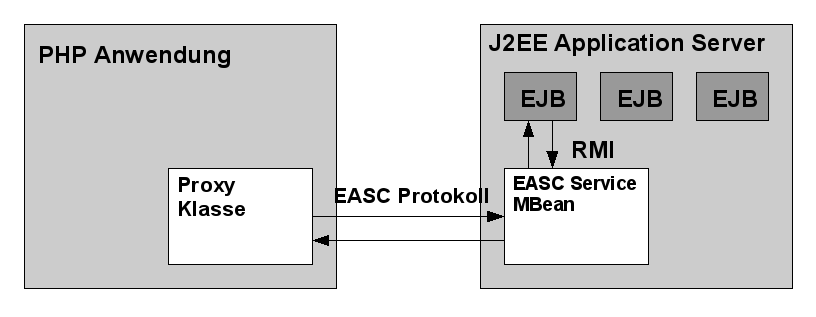
\includegraphics[width=\textwidth]{intro/img/easc.png}
\caption{EASC-Funktionsweise - nach \cite{EASC}}
\label{fig:easc}
\end{figure}

\section{php/Java bridge und die Java-Extension}
\label{sec:background:bridge}
Die php/Java bridge ist ein XML-basiertes Netzwerkprotokoll, das benutzt werden kann um einen PHP-Interpreter mit einer laufenden Java Virtual Machine
zu verbinden.
Die Java-Extension ist eine PHP-Extension\footnote{PHP-Erweiterung, siehe \ref{sec:background:php}} die dieses Protokoll benutzt um aus PHP heraus
in der JVM Objekte zu erzeugen, und die dann Stubs dieser Objekte in PHP verf"ugbar macht, was es dem PHP-Anwender erlaubt auf diesen Objekten
Methoden aufzurufen. Leider scheidet dieses Protokoll zur Implementierung der Aufgabe aus, erstens da es an den selben Nachteilen einer XML-Serialisierung
krankt wie beispielsweise auch SOAP, aber vor allem da es - "ahnlich wie EASC - den Zugriff von Java auf PHP nicht erm"oglicht. Weiterhin ist die
Java-Extension nicht mehr Teil des offiziellen PHP-Quelltextes, und wird auch nicht mehr gewartet, so ist es unter anderem nur sehr schwer
m"oglich die Extension in PHP 5 einzubinden.
N"aheres zur php/Java bridge findet man unter \cite{BRIDGEHP}.

\section{Java Native Interface - JNI}
\label{sec:background:JNI}

Java-Programme erreichen ihre Plattformunabh"angigkeit vorrangig dadurch, dass sie eine virtuelle Maschine (\emph{Java Virtual Machine - JVM}) vorraussetzen in welcher sie
ausgef"uhrt werden. Diese virtuelle Maschine verhindert allerdings zun"achst, dass beispielsweise plattformspezifische Funktionen oder vorhandene, nicht in Java
geschriebene Programmbibliotheken aus Java heraus angesprochen werden k"onnen.
Um dies zu umgehen bietet Java dem Entwickler mit dem JNI eine standardisierte M"oglichkeit zur Laufzeit betriebssystemspezifische Bibliotheken 
(.dll unter Windows, .so unter unixoiden Betriebssystemen) einzubinden und Funktionen beziehungsweise Methoden, welche diese bereitstellen, aufzurufen. 
JNI erm"oglicht nicht nur den Aufruf solcher Methoden aus Java heraus, sondern auch Aufrufe von Java-Methoden aus der eingebundenen Bibliothek heraus.
Native Funktionen werden in einer eigenen .c oder .cpp (C oder C++) Datei implementiert, wobei C++ eine etwas sauberere Verbindung mit dem JNI erlaubt.
Um aus Java heraus eine native Methode aufzurufen, muss diese im Javaquelltext als \texttt{native} deklariert werden. Aus der kompilierten Java-Klasse kann
mittels des Werkzeuges \emph{javah} eine Headerdatei erstellt werden, die die n"otige Funktionsdeklaration enth"alt. Mit Hilfe dieser Headerdatei kann
nun die native Programmbilbiothek entwickelt werden.
In der Java-Anwendung muss vor dem Aufruf der nativen Methode die entsprechende Programmbibliothek mittels \emph{System.loadLibray} geladen werden.

JNI wird unter anderem f"ur performance-kritische Zwecke (zum Beispiel in Grafikanwendungen) eingesetzt. Allerdings setzen auch viele im Java-Standard enthaltene
Klassen - wie beispielsweise jene, die f"ur die Audioausgabe oder f"ur Dateizugriffe zust"andig sind - JNI Implementierungen vorraus um auf diese
plattformspezifischen Funktionalit"aten in einer sicheren und kontrollierten Art und Weise zuzugreifen. Leider sichert JNI den Anwender nicht gegen s"amtliche m"oglichen
Fehler ab: zwar kann beim Aufruf der Bibliotheksfunktionen kein Fehler mehr begangen werden, allerdings k"onnen sich Programmierfehler innerhalb der
Bibliothek selbst weiterhin negativ auswirken, und zwar nicht nur auf den nativen Teil der Anwendung, sondern unter Umst"anden sogar auf die JVM selbst.

Mehr Informationen zum JNI sind unter Anderem auf der JNI-Homepage (\cite{JNIHP}), und in dem Buch "'Java Native Interface"' von Sheng Liang (\cite{JNIBOOK}) zu finden.


% ********** End of chapter **********
